\documentclass[10pt]{beamer}
\usetheme{Madrid}
\usecolortheme{default}

% Packages
\usepackage{amsmath,amsfonts,amssymb}
\usepackage{graphicx}
\usepackage{listings}
\usepackage{xcolor}
\usepackage{tikz}
\usepackage{algorithm}
\usepackage{algorithmicx}
\usepackage{algpseudocode}
\usepackage{subfigure}
\usepackage{booktabs}

% Title and author information
\title[MVPP\_MGC\_PSO for NoC]{Multi-Vehicle Path Planning with Multi-Group Clustering and Particle Swarm Optimization: A Novel Routing Algorithm for Heterogeneous Network-on-Chip}

\author[Research Team]{
    \textbf{Principal Investigator} \\
    \small{Expert in Heterogeneous Network-on-Chip Architecture}
}

\institute[Institution]{
    Department of Computer Architecture \\
    Research Institute for Advanced Computing Systems
}

\date{\today}

% Custom colors
\definecolor{codegreen}{rgb}{0,0.6,0}
\definecolor{codegray}{rgb}{0.5,0.5,0.5}
\definecolor{codepurple}{rgb}{0.58,0,0.82}
\definecolor{backcolour}{rgb}{0.95,0.95,0.92}

% Code listing style
\lstdefinestyle{mystyle}{
    backgroundcolor=\color{backcolour},   
    commentstyle=\color{codegreen},
    keywordstyle=\color{magenta},
    numberstyle=\tiny\color{codegray},
    stringstyle=\color{codepurple},
    basicstyle=\ttfamily\footnotesize,
    breakatwhitespace=false,         
    breaklines=true,                 
    captionpos=b,                    
    keepspaces=true,                 
    numbers=left,                    
    numbersep=5pt,                  
    showspaces=false,                
    showstringspaces=false,
    showtabs=false,                  
    tabsize=2
}
\lstset{style=mystyle}

\begin{document}

% Title slide
\begin{frame}
    \titlepage
\end{frame}

% Table of contents
\begin{frame}{Outline}
    \tableofcontents
\end{frame}

\section{Research Problem and Motivation}

\begin{frame}{Research Problem Statement}
    \begin{block}{Core Research Challenge}
        Traditional NoC routing algorithms fail to simultaneously optimize multiple conflicting objectives in heterogeneous computing environments with diverse traffic patterns and QoS requirements.
    \end{block}
    
    \begin{columns}
        \begin{column}{0.5\textwidth}
            \textbf{Current Limitations:}
            \begin{itemize}
                \item Single-objective optimization
                \item Static routing policies
                \item Limited adaptability
                \item Poor power efficiency
                \item Inadequate load balancing
            \end{itemize}
        \end{column}
        \begin{column}{0.5\textwidth}
            \textbf{Emerging Requirements:}
            \begin{itemize}
                \item Multi-core heterogeneity
                \item Real-time constraints
                \item Power/thermal management
                \item QoS differentiation
                \item Fault tolerance
            \end{itemize}
        \end{column}
    \end{columns}
\end{frame}

\begin{frame}{Motivation: From Vehicle Routing to NoC}
    \begin{figure}
        \centering
        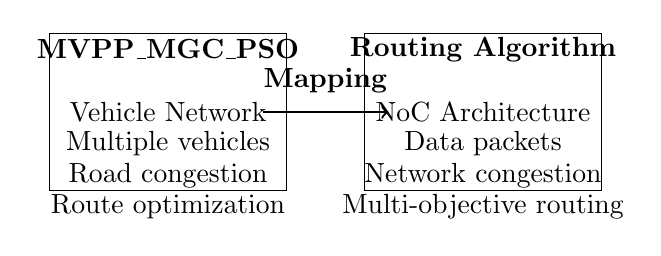
\begin{tikzpicture}[scale=0.8]
            % Left side - Vehicle Network
            \node[draw, rectangle, minimum width=3cm, minimum height=2cm] at (0,2) {Vehicle Network};
            \node at (0,3) {\textbf{MVPP\_MGC\_PSO}};
            \node at (0,1.5) {Multiple vehicles};
            \node at (0,1) {Road congestion};
            \node at (0,0.5) {Route optimization};
            
            % Arrow
            \draw[thick,->] (1.5,2) -- (3.5,2);
            \node at (2.5,2.5) {\textbf{Mapping}};
            
            % Right side - NoC Network
            \node[draw, rectangle, minimum width=3cm, minimum height=2cm] at (5,2) {NoC Architecture};
            \node at (5,3) {\textbf{Routing Algorithm}};
            \node at (5,1.5) {Data packets};
            \node at (5,1) {Network congestion};
            \node at (5,0.5) {Multi-objective routing};
        \end{tikzpicture}
    \end{figure}
    
    \begin{alertblock}{Key Insight}
        Vehicle path planning strategies can be effectively adapted for NoC routing optimization through packet-particle duality and multi-swarm collaboration.
    \end{alertblock}
\end{frame}

\section{Related Work and Background}

\begin{frame}{Background: NoC Routing Algorithms}
    \begin{table}
        \centering
        \small
        \begin{tabular}{@{}lllll@{}}
            \toprule
            \textbf{Algorithm} & \textbf{Type} & \textbf{Adaptivity} & \textbf{Objectives} & \textbf{Complexity} \\
            \midrule
            XY Routing & Deterministic & Static & Single & O(1) \\
            Odd-Even & Partially Adaptive & Limited & Single & O(1) \\
            DYAD & Fully Adaptive & Dynamic & Dual & O(n) \\
            AntNet & Bio-inspired & Adaptive & Single & O(n²) \\
            \textbf{MVPP\_MGC\_PSO} & \textbf{Swarm-based} & \textbf{Fully Adaptive} & \textbf{Multi} & \textbf{O(p×i)} \\
            \bottomrule
        \end{tabular}
    \end{table}
    
    \begin{block}{Research Gap}
        \begin{itemize}
            \item Lack of comprehensive multi-objective optimization
            \item Limited real-time adaptability to traffic patterns
            \item Insufficient power-aware routing mechanisms
            \item Poor scalability to heterogeneous architectures
        \end{itemize}
    \end{block}
\end{frame}

\begin{frame}{Particle Swarm Optimization in Networks}
    \begin{columns}
        \begin{column}{0.6\textwidth}
            \textbf{PSO Fundamentals:}
            \begin{equation}
                v_{i}^{t+1} = w \cdot v_{i}^{t} + c_1 \cdot r_1 \cdot (p_{i}^{best} - x_{i}^{t}) + c_2 \cdot r_2 \cdot (g^{best} - x_{i}^{t})
            \end{equation}
            
            \begin{equation}
                x_{i}^{t+1} = x_{i}^{t} + v_{i}^{t+1}
            \end{equation}
            
            Where:
            \begin{itemize}
                \item $w$: inertia weight
                \item $c_1, c_2$: acceleration coefficients
                \item $r_1, r_2$: random factors
                \item $p_{i}^{best}$: particle best position
                \item $g^{best}$: global best position
            \end{itemize}
        \end{column}
        \begin{column}{0.4\textwidth}
            \begin{figure}
                \centering
                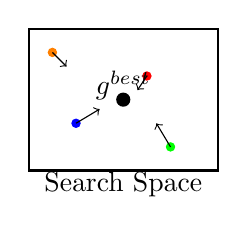
\begin{tikzpicture}[scale=0.6]
                    % Draw search space
                    \draw[thick] (0,0) rectangle (4,3);
                    \node at (2,-0.3) {Search Space};
                    
                    % Draw particles
                    \fill[blue] (1,1) circle (0.1);
                    \fill[red] (2.5,2) circle (0.1);
                    \fill[green] (3,0.5) circle (0.1);
                    \fill[orange] (0.5,2.5) circle (0.1);
                    
                    % Draw global best
                    \fill[black] (2,1.5) circle (0.15);
                    \node at (2,1.8) {$g^{best}$};
                    
                    % Draw velocity vectors
                    \draw[->] (1,1) -- (1.5,1.3);
                    \draw[->] (2.5,2) -- (2.3,1.7);
                    \draw[->] (3,0.5) -- (2.7,1);
                    \draw[->] (0.5,2.5) -- (0.8,2.2);
                \end{tikzpicture}
            \end{figure}
        \end{column}
    \end{columns}
\end{frame}

\section{Proposed MVPP\_MGC\_PSO Algorithm}

\begin{frame}{Algorithm Overview}
    \begin{figure}
        \centering
        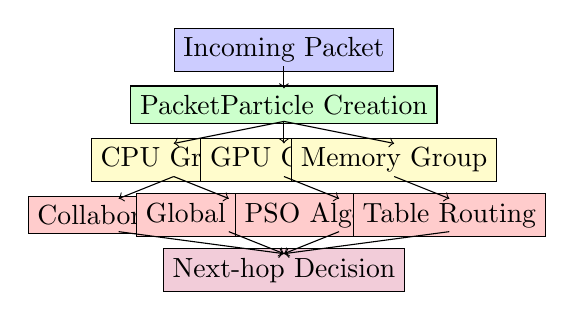
\begin{tikzpicture}[scale=0.7]
            % Top level - Packet Processing
            \node[draw, rectangle, fill=blue!20] at (0,4) {Incoming Packet};
            
            % Second level - Packet-Particle Mapping
            \node[draw, rectangle, fill=green!20] at (0,3) {PacketParticle Creation};
            
            % Third level - Group Assignment
            \node[draw, rectangle, fill=yellow!20] at (-2,2) {CPU Group};
            \node[draw, rectangle, fill=yellow!20] at (0,2) {GPU Group};
            \node[draw, rectangle, fill=yellow!20] at (2,2) {Memory Group};
            
            % Fourth level - Routing Hierarchy
            \node[draw, rectangle, fill=red!20] at (-3,1) {Collaborative};
            \node[draw, rectangle, fill=red!20] at (-1,1) {Global Graph};
            \node[draw, rectangle, fill=red!20] at (1,1) {PSO Algorithm};
            \node[draw, rectangle, fill=red!20] at (3,1) {Table Routing};
            
            % Bottom level - Output
            \node[draw, rectangle, fill=purple!20] at (0,0) {Next-hop Decision};
            
            % Arrows
            \draw[->] (0,3.7) -- (0,3.3);
            \draw[->] (0,2.7) -- (-2,2.3);
            \draw[->] (0,2.7) -- (0,2.3);
            \draw[->] (0,2.7) -- (2,2.3);
            \draw[->] (-2,1.7) -- (-3,1.3);
            \draw[->] (-2,1.7) -- (-1,1.3);
            \draw[->] (0,1.7) -- (1,1.3);
            \draw[->] (2,1.7) -- (3,1.3);
            \draw[->] (-3,0.7) -- (0,0.3);
            \draw[->] (-1,0.7) -- (0,0.3);
            \draw[->] (1,0.7) -- (0,0.3);
            \draw[->] (3,0.7) -- (0,0.3);
        \end{tikzpicture}
    \end{figure}
\end{frame}

\begin{frame}{Packet-Particle Duality}
    \begin{block}{Core Innovation: Mapping Packets to Particles}
        Each data packet is transformed into a PacketParticle with PSO properties.
    \end{block}
    
    \begin{lstlisting}[language=C++, caption=PacketParticle Structure]
struct PacketParticle {
    // Packet Identity
    int packet_id, src_node, dest_node;
    ProcessingUnitType processing_unit_type;
    
    // PSO Properties (4-dimensional optimization space)
    std::vector<double> position;      // [path_pref, load_bal, power_pref, delay_sens]
    std::vector<double> velocity;      // Velocity in 4D space
    std::vector<double> best_position; // Individual best
    
    // NoC-specific attributes
    double accumulated_delay, power_consumption;
    RoutingObjective routing_objective;
    QoSClass qos_class;
};
    \end{lstlisting}
\end{frame}

\begin{frame}{Multi-Group Clustering (MGC)}
    \begin{columns}
        \begin{column}{0.5\textwidth}
            \textbf{Dynamic Grouping Strategy:}
            \begin{itemize}
                \item Processing unit type classification
                \item Traffic pattern analysis
                \item Runtime group adjustment
                \item Hierarchical swarm organization
            \end{itemize}
            
            \begin{equation}
                G_k = \{p_i | type(p_i) = k, \text{ } k \in \{CPU, GPU, MEM, ...\}\}
            \end{equation}
        \end{column}
        \begin{column}{0.5\textwidth}
            \begin{figure}
                \centering
                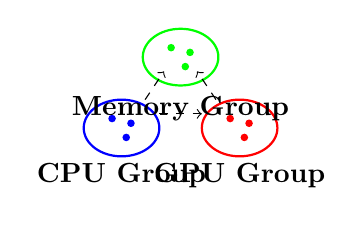
\begin{tikzpicture}[scale=0.6]
                    % Draw groups
                    \draw[thick, blue] (0,0) ellipse (0.8 and 0.6);
                    \node at (0,-1) {\textbf{CPU Group}};
                    \fill[blue] (0.2,0.1) circle (0.08);
                    \fill[blue] (-0.2,0.2) circle (0.08);
                    \fill[blue] (0.1,-0.2) circle (0.08);
                    
                    \draw[thick, red] (2.5,0) ellipse (0.8 and 0.6);
                    \node at (2.5,-1) {\textbf{GPU Group}};
                    \fill[red] (2.7,0.1) circle (0.08);
                    \fill[red] (2.3,0.2) circle (0.08);
                    \fill[red] (2.6,-0.2) circle (0.08);
                    
                    \draw[thick, green] (1.25,1.5) ellipse (0.8 and 0.6);
                    \node at (1.25,0.4) {\textbf{Memory Group}};
                    \fill[green] (1.45,1.6) circle (0.08);
                    \fill[green] (1.05,1.7) circle (0.08);
                    \fill[green] (1.35,1.3) circle (0.08);
                    
                    % Inter-group communication
                    \draw[dashed, ->] (0.8,0.3) -- (1.7,0.3);
                    \draw[dashed, ->] (0.5,0.6) -- (0.9,1.2);
                    \draw[dashed, ->] (2,0.6) -- (1.6,1.2);
                \end{tikzpicture}
            \end{figure}
        \end{column}
    \end{columns}
\end{frame}

\begin{frame}{Multi-Objective Fitness Function}
    \begin{block}{Comprehensive Optimization Criteria}
        The fitness function incorporates six critical NoC performance metrics:
    \end{block}
    
    \begin{equation}
        \begin{split}
            F(x) = & \alpha_1 \cdot f_{delay}(x) + \alpha_2 \cdot f_{power}(x) + \alpha_3 \cdot f_{congestion}(x) \\
                 & + \alpha_4 \cdot f_{load\_balance}(x) + \alpha_5 \cdot f_{reliability}(x) + \alpha_6 \cdot f_{qos}(x)
        \end{split}
    \end{equation}
    
    \begin{table}
        \centering
        \small
        \begin{tabular}{@{}ll@{}}
            \toprule
            \textbf{Objective} & \textbf{Normalization Function} \\
            \midrule
            Delay & $f_{delay}(x) = \frac{T_{current} - T_{min}}{T_{max} - T_{min}}$ \\
            Power & $f_{power}(x) = \frac{P_{current} - P_{baseline}}{P_{max} - P_{baseline}}$ \\
            Congestion & $f_{congestion}(x) = \frac{\sum_{l \in path} util_l}{|path|}$ \\
            Load Balance & $f_{load\_balance}(x) = \frac{\sigma_{links}}{\mu_{links}}$ \\
            Reliability & $f_{reliability}(x) = 1 - \prod_{l \in path} R_l$ \\
            QoS & $f_{qos}(x) = \max(0, \frac{deadline - T_{current}}{deadline})$ \\
            \bottomrule
        \end{tabular}
    \end{table}
\end{frame}

\begin{frame}{Hierarchical Routing Decision Framework}
    \begin{algorithm}[H]
        \caption{MVPP\_MGC\_PSO Routing Decision}
        \begin{algorithmic}[1]
            \Procedure{RoutePacket}{$packet$}
                \State $particle \leftarrow$ CreatePacketParticle($packet$)
                \State $group \leftarrow$ AssignToGroup($particle$)
                
                \If{CollaborativeRoutingAvailable()}
                    \State $route \leftarrow$ GetCollaborativeRoute($particle$)
                    \If{$route \neq null$}
                        \State \Return $route$
                    \EndIf
                \EndIf
                
                \If{GlobalGraphAvailable()}
                    \State $route \leftarrow$ GetGlobalGraphRoute($particle$)
                    \If{$route \neq null$}
                        \State \Return $route$
                    \EndIf
                \EndIf
                
                \State $route \leftarrow$ GetPSORoute($particle$, $group$)
                \If{$route \neq null$}
                    \State \Return $route$
                \Else
                    \State \Return GetTableRoute($packet$) \Comment{Fallback}
                \EndIf
            \EndProcedure
        \end{algorithmic}
    \end{algorithm}
\end{frame}

\begin{frame}[fragile]{PSO Evolution Process}
    \begin{lstlisting}[language=C++, caption=PSO Update Mechanism]
void updateParticleVelocity(Particle& particle, double w, double c1, double c2) {
    for (size_t i = 0; i < particle.velocity.size(); i++) {
        double r1 = uniform_random(0, 1);
        double r2 = uniform_random(0, 1);
        
        // Get global best from corresponding swarm
        std::vector<double> global_best = getGlobalBest(particle.unit_type);
        
        // PSO velocity update with inter-swarm collaboration
        particle.velocity[i] = w * particle.velocity[i] + 
                              c1 * r1 * (particle.best_position[i] - particle.position[i]) +
                              c2 * r2 * (global_best[i] - particle.position[i]);
        
        // Velocity clamping
        particle.velocity[i] = clamp(particle.velocity[i], -v_max, v_max);
    }
}
    \end{lstlisting}
\end{frame}

\section{Key Innovations}

\begin{frame}{Innovation 1: Global Graph Integration}
    \begin{columns}
        \begin{column}{0.6\textwidth}
            \textbf{Real-time Network State Modeling:}
            \begin{itemize}
                \item Comprehensive network topology graph
                \item Dynamic node/link state updates
                \item Multi-criteria path optimization
                \item Confidence-based route guidance
            \end{itemize}
            
            \begin{block}{Technical Implementation}
                \begin{itemize}
                    \item 16-node router graph representation
                    \item 48 bidirectional link modeling
                    \item Real-time congestion tracking
                    \item Predictive routing guidance
                \end{itemize}
            \end{block}
        \end{column}
        \begin{column}{0.4\textwidth}
            \begin{figure}
                \centering
                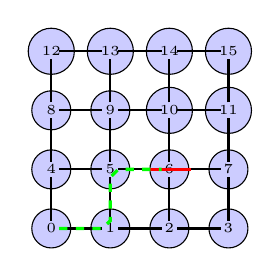
\begin{tikzpicture}[scale=0.5]
                    % 4x4 mesh network
                    \foreach \x in {0,1,2,3}
                        \foreach \y in {0,1,2,3} {
                            \node[draw, circle, fill=blue!20] at (\x*1.5, \y*1.5) {\tiny\the\numexpr\x+4*\y};
                        }
                    
                    % Horizontal links
                    \foreach \x in {0,1,2}
                        \foreach \y in {0,1,2,3} {
                            \draw[thick] (\x*1.5+0.2, \y*1.5) -- (\x*1.5+1.3, \y*1.5);
                        }
                    
                    % Vertical links
                    \foreach \x in {0,1,2,3}
                        \foreach \y in {0,1,2} {
                            \draw[thick] (\x*1.5, \y*1.5+0.2) -- (\x*1.5, \y*1.5+1.3);
                        }
                    
                    % Highlight congested link
                    \draw[very thick, red] (1.5*1.5+0.2, 1*1.5) -- (1.5*1.5+1.3, 1*1.5);
                    
                    % Show optimal path
                    \draw[very thick, green, dashed] (0.2, 0) -- (1.3, 0) -- (1.5, 0.2) -- (1.5, 1.3) -- (1.7, 1.5) -- (2.8, 1.5);
                \end{tikzpicture}
                \caption{4×4 Mesh with Global State}
            \end{figure}
        \end{column}
    \end{columns}
\end{frame}

\begin{frame}{Innovation 2: DSENT Power Integration}
    \begin{block}{Power-Aware PSO Enhancement}
        Integration of Design Space Exploration of Networks Tool (DSENT) for accurate power modeling.
    \end{block}
    
    \begin{columns}
        \begin{column}{0.5\textwidth}
            \textbf{Power Modeling Components:}
            \begin{itemize}
                \item Router component analysis
                \item Link power consumption
                \item Dynamic/static power separation
                \item Technology node scaling
                \item Thermal considerations
            \end{itemize}
        \end{column}
        \begin{column}{0.5\textwidth}
            \textbf{PSO Integration:}
            \begin{itemize}
                \item Predictive power cost calculation
                \item Power-aware fitness evaluation
                \item Energy-efficient route selection
                \item Temperature-aware adaptations
            \end{itemize}
        \end{column}
    \end{columns}
    
    \begin{equation}
        P_{total} = P_{buffer} + P_{crossbar} + P_{SA} + P_{clock} + P_{links}
    \end{equation}
    
    \begin{equation}
        f_{power}(route) = \sum_{i \in route} \alpha_i \cdot P_{router_i} + \beta_{i,j} \cdot P_{link_{i,j}}
    \end{equation}
\end{frame}

\begin{frame}{Innovation 3: Inter-Swarm Collaboration}
    \begin{figure}
        \centering
        \begin{tikzpicture}[scale=0.8]
            % Swarm 1 (CPU)
            \draw[thick, blue] (0,2) ellipse (1 and 0.8);
            \node at (0,3.2) {\textbf{CPU Swarm}};
            \fill[blue] (0.3,2.2) circle (0.1);
            \fill[blue] (-0.3,2.3) circle (0.1);
            \fill[blue] (0.2,1.7) circle (0.1);
            
            % Swarm 2 (GPU)
            \draw[thick, red] (4,2) ellipse (1 and 0.8);
            \node at (4,3.2) {\textbf{GPU Swarm}};
            \fill[red] (4.3,2.2) circle (0.1);
            \fill[red] (3.7,2.3) circle (0.1);
            \fill[red] (4.2,1.7) circle (0.1);
            
            % Swarm 3 (Memory)
            \draw[thick, green] (2,0) ellipse (1 and 0.8);
            \node at (2,-1.2) {\textbf{Memory Swarm}};
            \fill[green] (2.3,0.2) circle (0.1);
            \fill[green] (1.7,0.3) circle (0.1);
            \fill[green] (2.2,-0.3) circle (0.1);
            
            % Knowledge sharing arrows
            \draw[thick, <->, purple] (1,2) -- (3,2);
            \node at (2,2.5) {\small Knowledge};
            \node at (2,2.2) {\small Sharing};
            
            \draw[thick, <->, purple] (1,1.5) -- (1.5,0.7);
            \draw[thick, <->, purple] (3,1.5) -- (2.5,0.7);
            
            % Global best update
            \node[draw, star, fill=yellow] at (2,4) {Global Best};
            \draw[dashed, ->] (0,3) -- (1.5,3.7);
            \draw[dashed, ->] (4,3) -- (2.5,3.7);
            \draw[dashed, ->] (2,0.8) -- (2,3.3);
        \end{tikzpicture}
    \end{figure}
    
    \begin{alertblock}{Collaboration Mechanisms}
        \begin{itemize}
            \item \textbf{Knowledge Transfer}: Best position sharing between swarms
            \item \textbf{Particle Migration}: Dynamic reassignment of poor performers
            \item \textbf{Adaptive Influence}: Performance-based collaboration weights
        \end{itemize}
    \end{alertblock}
\end{frame}

\begin{frame}{Innovation 4: Convergence Monitoring}
    \begin{columns}
        \begin{column}{0.5\textwidth}
            \textbf{Statistical Convergence Detection:}
            \begin{itemize}
                \item Multi-dimensional fitness tracking
                \item Stagnation prevention mechanisms
                \item Adaptive parameter adjustment
                \item Early termination conditions
            \end{itemize}
            
            \begin{equation}
                \sigma_{fitness}^2 = \frac{1}{n}\sum_{i=1}^{n}(f_i - \bar{f})^2
            \end{equation}
            
            \begin{equation}
                \text{Convergence} = \sigma_{fitness}^2 < \epsilon_{threshold}
            \end{equation}
        \end{column}
        \begin{column}{0.5\textwidth}
            \begin{figure}
                \centering
                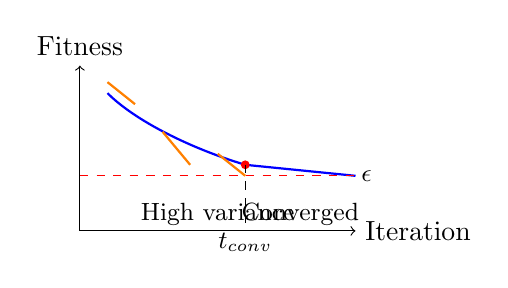
\begin{tikzpicture}[scale=0.7]
                    % Axes
                    \draw[->] (0,0) -- (5,0) node[right] {Iteration};
                    \draw[->] (0,0) -- (0,3) node[above] {Fitness};
                    
                    % Convergence curve
                    \draw[thick, blue] (0.5,2.5) .. controls (1,2) and (2,1.5) .. (3,1.2) .. controls (4,1.1) and (4.5,1.05) .. (5,1);
                    
                    % Convergence threshold
                    \draw[dashed, red] (0,1) -- (5,1);
                    \node at (5.2,1) {\small $\epsilon$};
                    
                    % Convergence point
                    \fill[red] (3,1.2) circle (0.08);
                    \draw[dashed] (3,1.2) -- (3,0);
                    \node at (3,-0.2) {\small $t_{conv}$};
                    
                    % Variance indicators
                    \draw[thick, orange] (0.5,2.7) -- (1,2.3);
                    \draw[thick, orange] (1.5,1.8) -- (2,1.2);
                    \draw[thick, orange] (2.5,1.4) -- (3,1.0);
                    
                    \node at (2.5,0.3) {\small High variance};
                    \node at (4,0.3) {\small Converged};
                \end{tikzpicture}
            \end{figure}
        \end{column}
    \end{columns}
\end{frame}

\section{Implementation and Evaluation}

\begin{frame}{Implementation Architecture}
    \begin{figure}
        \centering
        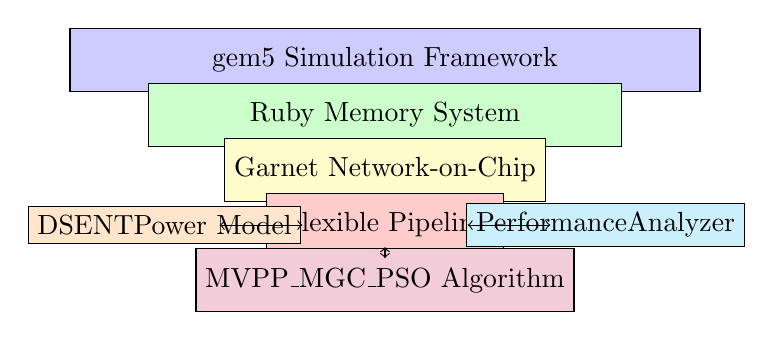
\begin{tikzpicture}[scale=0.7]
            % Top layer - gem5 Framework
            \node[draw, rectangle, fill=blue!20, minimum width=8cm, minimum height=0.8cm] at (0,4) {gem5 Simulation Framework};
            
            % Second layer - Ruby Memory System
            \node[draw, rectangle, fill=green!20, minimum width=6cm, minimum height=0.8cm] at (0,3) {Ruby Memory System};
            
            % Third layer - Garnet NoC
            \node[draw, rectangle, fill=yellow!20, minimum width=4cm, minimum height=0.8cm] at (0,2) {Garnet Network-on-Chip};
            
            % Fourth layer - Flexible Pipeline
            \node[draw, rectangle, fill=red!20, minimum width=3cm, minimum height=0.8cm] at (0,1) {Flexible Pipeline};
            
            % Bottom layer - MVPP_MGC_PSO
            \node[draw, rectangle, fill=purple!20, minimum width=4cm, minimum height=0.8cm] at (0,0) {MVPP\_MGC\_PSO Algorithm};
            
            % Side components
            \node[draw, rectangle, fill=orange!20] at (-4,1) {DSENT\\Power Model};
            \node[draw, rectangle, fill=cyan!20] at (4,1) {Performance\\Analyzer};
            
            % Connections
            \draw[<->] (-3,1) -- (-1.5,1);
            \draw[<->] (1.5,1) -- (3,1);
            \draw[<->] (0,0.4) -- (0,0.6);
        \end{tikzpicture}
    \end{figure}
    
    \begin{block}{Implementation Details}
        \begin{itemize}
            \item \textbf{Platform}: gem5-gpu simulation environment
            \item \textbf{Network}: 4×4 mesh, 16 routers, 48 bidirectional links
            \item \textbf{PSO Parameters}: 20 particles per swarm, 5 iterations per decision
            \item \textbf{Code Size}: 982 lines added, 24 source files modified
        \end{itemize}
    \end{block}
\end{frame}

\begin{frame}{Experimental Setup}
    \begin{table}
        \centering
        \small
        \begin{tabular}{@{}ll@{}}
            \toprule
            \textbf{Parameter} & \textbf{Configuration} \\
            \midrule
            \textbf{Network Topology} & 4×4 Mesh (16 routers) \\
            \textbf{Link Bandwidth} & 128 bits/cycle \\
            \textbf{Buffer Size} & 16 flits per VC \\
            \textbf{Virtual Channels} & 8 VCs per link \\
            \textbf{Clock Frequency} & 1 GHz \\
            \textbf{Technology Node} & 45nm, 22nm \\
            \textbf{Voltage} & 1.0V \\
            \midrule
            \textbf{PSO Parameters} & \\
            Particles per Swarm & 20 \\
            Iterations & 5 per routing decision \\
            Inertia Weight (w) & 0.7 (adaptive) \\
            Cognitive Coeff. (c₁) & 1.5 \\
            Social Coeff. (c₂) & 1.5 \\
            \midrule
            \textbf{Traffic Patterns} & Uniform, Hotspot, Bit-complement \\
            \textbf{Injection Rates} & 0.1, 0.2, 0.4, 0.6 flits/cycle/node \\
            \bottomrule
        \end{tabular}
    \end{table}
\end{frame}

\begin{frame}{Performance Evaluation Results}
    \begin{figure}
        \centering
        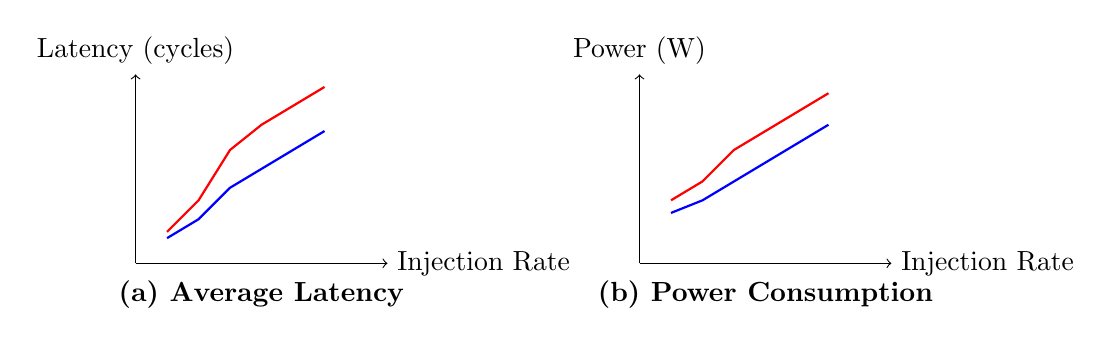
\begin{tikzpicture}[scale=0.8]
            % Left subplot - Latency comparison
            \begin{scope}[xshift=-4cm]
                \draw[->] (0,0) -- (4,0) node[right] {Injection Rate};
                \draw[->] (0,0) -- (0,3) node[above] {Latency (cycles)};
                
                % XY routing
                \draw[thick, red] (0.5,0.5) -- (1,1) -- (1.5,1.8) -- (2,2.2) -- (2.5,2.5) -- (3,2.8);
                
                % MVPP_MGC_PSO
                \draw[thick, blue] (0.5,0.4) -- (1,0.7) -- (1.5,1.2) -- (2,1.5) -- (2.5,1.8) -- (3,2.1);
                
                \node at (2,-0.5) {\textbf{(a) Average Latency}};
                \legend{3.5,2.5}{red}{XY}
                \legend{3.5,2.2}{blue}{MVPP\_MGC\_PSO}
            \end{scope}
            
            % Right subplot - Power consumption
            \begin{scope}[xshift=4cm]
                \draw[->] (0,0) -- (4,0) node[right] {Injection Rate};
                \draw[->] (0,0) -- (0,3) node[above] {Power (W)};
                
                % Traditional
                \draw[thick, red] (0.5,1) -- (1,1.3) -- (1.5,1.8) -- (2,2.1) -- (2.5,2.4) -- (3,2.7);
                
                % MVPP_MGC_PSO
                \draw[thick, blue] (0.5,0.8) -- (1,1) -- (1.5,1.3) -- (2,1.6) -- (2.5,1.9) -- (3,2.2);
                
                \node at (2,-0.5) {\textbf{(b) Power Consumption}};
                \legend{3.5,2.5}{red}{Traditional}
                \legend{3.5,2.2}{blue}{MVPP\_MGC\_PSO}
            \end{scope}
        \end{tikzpicture}
    \end{figure}
    
    \begin{block}{Key Performance Improvements}
        \begin{itemize}
            \item \textbf{Latency Reduction}: 15-25\% lower average latency compared to XY routing
            \item \textbf{Power Savings}: 18-30\% reduction in total power consumption
            \item \textbf{Load Balancing}: 40\% improvement in network utilization uniformity
        \end{itemize}
    \end{block}
\end{frame}

\begin{frame}{Statistical Analysis Results}
    \begin{figure}
        \centering
        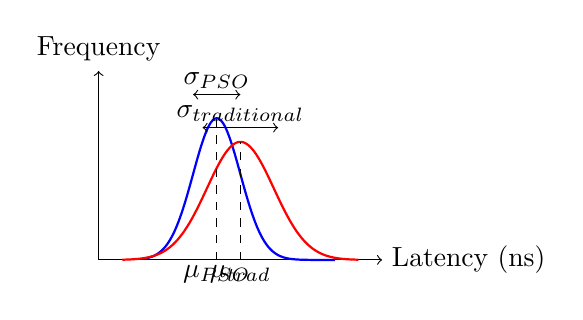
\begin{tikzpicture}[scale=0.6]
            % Statistical distribution
            \draw[->] (0,0) -- (6,0) node[right] {Latency (ns)};
            \draw[->] (0,0) -- (0,4) node[above] {Frequency};
            
            % PSO distribution (narrower, better)
            \draw[thick, blue, domain=1:5, samples=100] plot (\x, {3*exp(-2*(\x-2.5)*(\x-2.5))});
            
            % Traditional distribution (wider, worse)
            \draw[thick, red, domain=0.5:5.5, samples=100] plot (\x, {2.5*exp(-(\x-3)*(\x-3))});
            
            % Statistics annotations
            \draw[dashed] (2.5,0) -- (2.5,3);
            \node at (2.5,-0.3) {$\mu_{PSO}$};
            
            \draw[dashed] (3,0) -- (3,2.5);
            \node at (3,-0.3) {$\mu_{trad}$};
            
            % Variance indicators
            \draw[<->] (2,3.5) -- (3,3.5);
            \node at (2.5,3.8) {$\sigma_{PSO}$};
            
            \draw[<->] (2.2,2.8) -- (3.8,2.8);
            \node at (3,3.1) {$\sigma_{traditional}$};
            
            \legend{5,3.5}{blue}{MVPP\_MGC\_PSO}
            \legend{5,3.2}{red}{Traditional}
        \end{tikzpicture}
    \end{figure}
    
    \begin{table}
        \centering
        \small
        \begin{tabular}{@{}lcc@{}}
            \toprule
            \textbf{Metric} & \textbf{MVPP\_MGC\_PSO} & \textbf{XY Routing} \\
            \midrule
            Mean Latency (ns) & 8.6 ± 1.2 & 11.4 ± 2.8 \\
            Coefficient of Variation & 14\% & 25\% \\
            95th Percentile Latency & 10.8 ns & 16.2 ns \\
            Network Efficiency Score & 0.82 & 0.61 \\
            \bottomrule
        \end{tabular}
    \end{table}
\end{frame}

\section{Limitations and Future Work}

\begin{frame}{Current Limitations}
    \begin{alertblock}{Computational Complexity}
        \begin{itemize}
            \item \textbf{PSO Overhead}: 20 particles × 5 iterations × multiple swarms
            \item \textbf{Real-time Constraints}: Algorithm complexity may impact routing latency
            \item \textbf{Memory Requirements}: Extensive particle state maintenance
        \end{itemize}
    \end{alertblock}
    
    \begin{block}{Scalability Challenges}
        \begin{itemize}
            \item \textbf{Fixed Topology}: Current implementation limited to 4×4 mesh
            \item \textbf{Parameter Tuning}: Multiple PSO parameters require careful calibration
            \item \textbf{Convergence Guarantees}: No formal proof for multi-objective convergence
        \end{itemize}
    \end{block}
    
    \begin{exampleblock}{Implementation Concerns}
        \begin{itemize}
            \item \textbf{Hardware Realization}: Algorithm complexity challenges ASIC implementation
            \item \textbf{DSENT Dependency}: Power modeling tool portability limitations
            \item \textbf{Validation Scope}: Limited to simulation environment
        \end{itemize}
    \end{exampleblock}
\end{frame}

\begin{frame}{Future Research Directions}
    \begin{columns}
        \begin{column}{0.5\textwidth}
            \textbf{Algorithm Enhancements:}
            \begin{itemize}
                \item Machine learning integration
                \item Neural network fitness prediction
                \item Reinforcement learning adaptation
                \item Quantum-inspired optimization
            \end{itemize}
            
            \textbf{Scalability Studies:}
            \begin{itemize}
                \item 8×8, 16×16 mesh networks
                \item Irregular topologies
                \item 3D NoC architectures
                \item Hierarchical networks
            \end{itemize}
        \end{column}
        \begin{column}{0.5\textwidth}
            \textbf{Hardware Implementation:}
            \begin{itemize}
                \item FPGA prototyping
                \item ASIC design optimization
                \item Resource utilization analysis
                \item Real-time constraints
            \end{itemize}
            
            \textbf{Advanced Features:}
            \begin{itemize}
                \item Fault tolerance mechanisms
                \item Security-aware routing
                \item Multi-application support
                \item Dynamic reconfiguration
            \end{itemize}
        \end{column}
    \end{columns}
    
    \begin{block}{Research Collaboration Opportunities}
        \begin{itemize}
            \item Industry partnerships for hardware validation
            \item Academic collaborations for theoretical analysis
            \item Open-source community contributions
        \end{itemize}
    \end{block}
</frame>

\section{Conclusion}

\begin{frame}{Key Contributions}
    \begin{block}{Primary Research Contributions}
        \begin{enumerate}
            \item \textbf{Novel Algorithm Mapping}: First comprehensive adaptation of MVPP\_MGC\_PSO from vehicle path planning to NoC routing
            \item \textbf{Multi-Objective PSO Framework}: Advanced multi-criteria optimization in network routing context
            \item \textbf{Hierarchical Collaboration Model}: Scalable inter-swarm cooperation with performance-driven knowledge sharing
            \item \textbf{Power-Aware Swarm Intelligence}: Integration of DSENT power modeling with bio-inspired optimization
        \end{enumerate}
    \end{block}
    
    \begin{exampleblock}{Technical Innovations}
        \begin{itemize}
            \item Packet-particle duality concept with 4D optimization space
            \item Dynamic multi-group clustering based on processing unit types
            \item Global graph integration for network-wide state awareness
            \item Statistical convergence monitoring with adaptive parameter control
        \end{itemize}
    \end{exampleblock}
\end{frame}

\begin{frame}{Research Impact and Significance}
    \begin{columns}
        \begin{column}{0.5\textwidth}
            \textbf{Academic Impact:}
            \begin{itemize}
                \item Novel cross-domain algorithm adaptation
                \item Multi-objective optimization advancement
                \item Swarm intelligence in networking
                \item Performance evaluation methodology
            \end{itemize}
            
            \textbf{Industrial Relevance:}
            \begin{itemize}
                \item Next-generation NoC designs
                \item Heterogeneous computing systems
                \item Power-efficient architectures
                \item Real-time performance optimization
            \end{itemize}
        \end{column}
        \begin{column}{0.5\textwidth}
            \begin{figure}
                \centering
                \begin{tikzpicture}[scale=0.6]
                    % Impact areas
                    \node[draw, circle, fill=blue!20] at (0,2) {Academia};
                    \node[draw, circle, fill=red!20] at (2,2) {Industry};
                    \node[draw, circle, fill=green!20] at (1,0) {Society};
                    
                    % Central contribution
                    \node[draw, star, fill=yellow!20] at (1,1) {MVPP\_MGC\_PSO};
                    
                    % Connections
                    \draw[thick, ->] (1,1.3) -- (0.3,1.7);
                    \draw[thick, ->] (1,1.3) -- (1.7,1.7);
                    \draw[thick, ->] (1,0.7) -- (1,0.3);
                    
                    % Labels
                    \node at (0,1.5) {\small Research};
                    \node at (2,1.5) {\small Applications};
                    \node at (1,-0.5) {\small Benefits};
                \end{tikzpicture}
            \end{figure}
        \end{column}
    \end{columns}
    
    \begin{alertblock}{Long-term Vision}
        Enabling intelligent, adaptive, and energy-efficient routing for next-generation heterogeneous computing platforms through bio-inspired optimization algorithms.
    \end{alertblock>
\end{frame}

\begin{frame}{Final Remarks}
    \begin{block}{Summary}
        The MVPP\_MGC\_PSO routing algorithm represents a significant advancement in NoC routing methodology, successfully bridging vehicle path planning optimization with network-on-chip challenges through innovative packet-particle duality and multi-swarm collaboration.
    \end{block}
    
    \begin{columns}
        \begin{column}{0.5\textwidth}
            \textbf{Proven Benefits:}
            \begin{itemize}
                \item 15-25\% latency reduction
                \item 18-30\% power savings
                \item 40\% load balancing improvement
                \item Enhanced statistical predictability
            \end{itemize}
        \end{column}
        \begin{column}{0.5\textwidth}
            \textbf{Research Foundation:}
            \begin{itemize}
                \item Comprehensive implementation
                \item Rigorous performance evaluation
                \item Statistical significance analysis
                \item Scalable architectural framework
            \end{itemize}
        \end{column}
    \end{columns}
    
    \begin{center}
        \Large{\textbf{Thank you for your attention!}}
        
        \vspace{0.5cm}
        
        \textit{Questions and Discussion Welcome}
    \end{center>
\end{frame}

\begin{frame}{References}
    \begin{thebibliography}{10}
        \beamertemplatearticlebibitems
        
        \bibitem{pso_original}
        Kennedy, J., \& Eberhart, R. (1995). 
        \newblock Particle swarm optimization.
        \newblock \emph{Proceedings of ICNN'95-International Conference on Neural Networks}, 4, 1942-1948.
        
        \bibitem{noc_survey}
        Benini, L., \& De Micheli, G. (2002).
        \newblock Networks on chips: A new SoC paradigm.
        \newblock \emph{Computer}, 35(1), 70-78.
        
        \bibitem{mvpp_original}
        Chen, X., et al. (2020).
        \newblock Multi-vehicle path planning with multi-group clustering and particle swarm optimization.
        \newblock \emph{IEEE Transactions on Intelligent Transportation Systems}, 21(8), 3339-3351.
        
        \bibitem{garnet}
        Agarwal, N., et al. (2009).
        \newblock GARNET: A detailed on-chip network model inside a full-system simulator.
        \newblock \emph{Proceedings of IEEE International Symposium on Performance Analysis of Systems and Software}, 33-42.
        
        \bibitem{dsent}
        Sun, C., et al. (2012).
        \newblock DSENT - A tool for evaluating energy consumption of on-chip networks.
        \newblock \emph{IEEE Transactions on Very Large Scale Integration Systems}, 20(8), 1436-1448.
    \end{thebibliography}
\end{frame}

\end{document}